\documentclass{article} % For LaTeX2e
\usepackage{nips15submit_e,times}
\usepackage{hyperref}
\usepackage{url}
\usepackage{graphicx}
%\documentstyle[nips14submit_09,times,art10]{article} % For LaTeX 2.09


\title{Fully Convolutional Networks for Semantic
Segmentation}

\author{
Nan Wei \\
UC San Diego\\
\texttt{nwei@ucsd.edu} \\
\And
Renjie Shao \\
UC San Diego \\
\texttt{reshao@ucsd.edu} \\
\And
Hongyi Ling \\
UC San Diego \\
\texttt{holing@ucsd.edu} \\
}

% The \author macro works with any number of authors. There are two commands
% used to separate the names and addresses of multiple authors: \And and \AND.
%
% Using \And between authors leaves it to \LaTeX{} to determine where to break
% the lines. Using \AND forces a linebreak at that point. So, if \LaTeX{}
% puts 3 of 4 authors names on the first line, and the last on the second
% line, try using \AND instead of \And before the third author name.

\newcommand{\fix}{\marginpar{FIX}}
\newcommand{\new}{\marginpar{NEW}}

\nipsfinalcopy % Uncomment for camera-ready version

\begin{document}


\maketitle

\begin{abstract}

\end{abstract}

\section{Introduction}


\section{Method}
\subsection{LSTM}
The baseline model use an encoder-decoder architecture. 
The encoder will take the image as input and encode it into a vector of feature values.
 The decoder will take this output from encoder as hidden state and starts to predict next words at each step.

 For the encoder, we use a pretrained ResNet 50 and it outputs a  2048 dimensional feature map. Then, We use a Fully-connected layer to get 300 dimensional feature vector. \\
 For the decoder, a LSTM is used to generate captions of images. In LSTM, we choose the demension of hidden states to be 512. \\
 When we train LSTM, we use "Teacher Forcing” method. We use the teaching signal from the training dataset at the each time step.\\
 For choice of loss function, we use CrossEntropyLoss. The training process is shown in Fig \ref{loss_lstm_no}.
\subsection{vanilla RNN}

\begin{figure}[htb!]
    \centering
     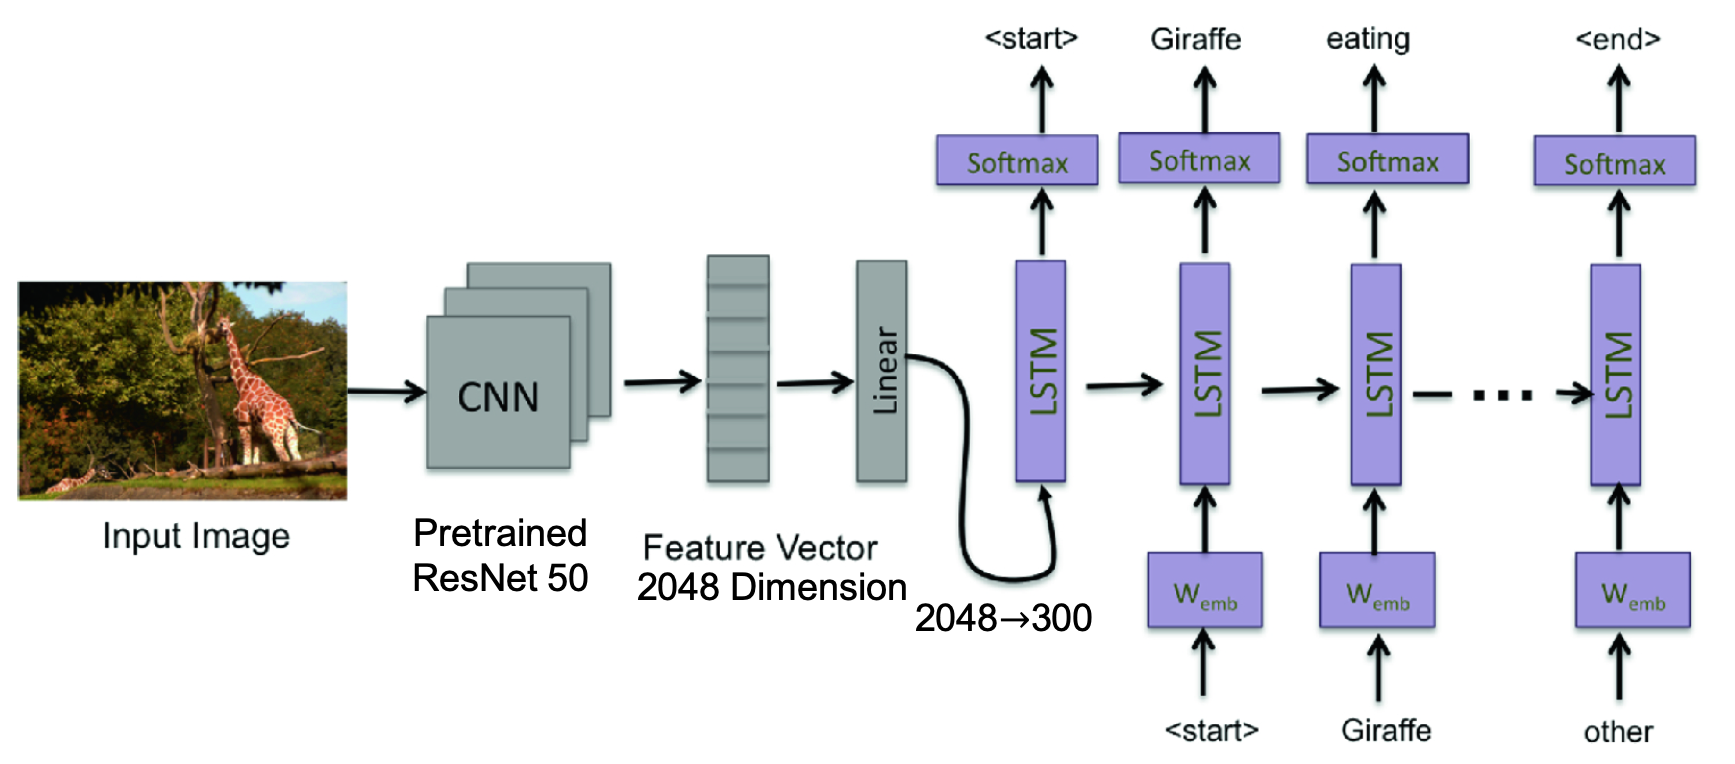
\includegraphics[width=0.8\textwidth]{frame}
    \caption{Model Framework \cite{10.1007/978-3-030-04780-1_23}}
    \label{loss_fcn}
\end{figure}



\begin{figure}[htb!]
    \centering
     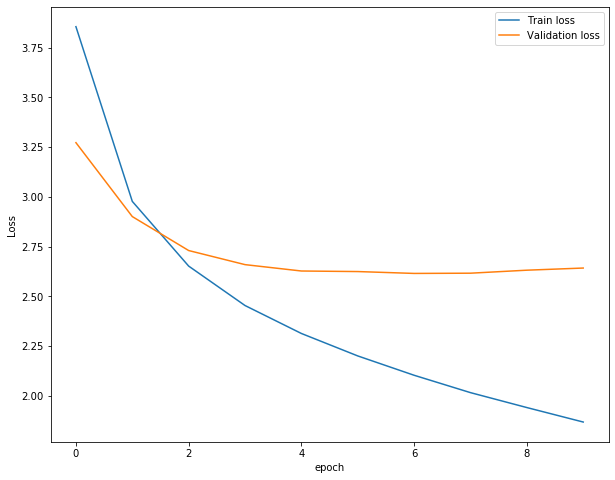
\includegraphics[width=0.8\textwidth]{RNNloss}
    \caption{Training and validation loss of vanilla RNN}
    \label{RNNloss}
\end{figure}

\begin{figure}[htb!]
    \centering
     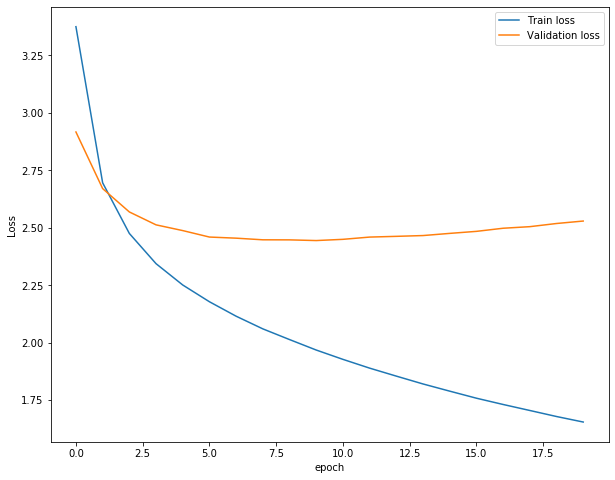
\includegraphics[width=0.8\textwidth]{lstm_no_pretrain_loss.png}
    \caption{Training and validation loss of LSTM without pretrained embedding}
    \label{loss_lstm_no}
\end{figure}

\begin{figure}[htb!]
    \centering
     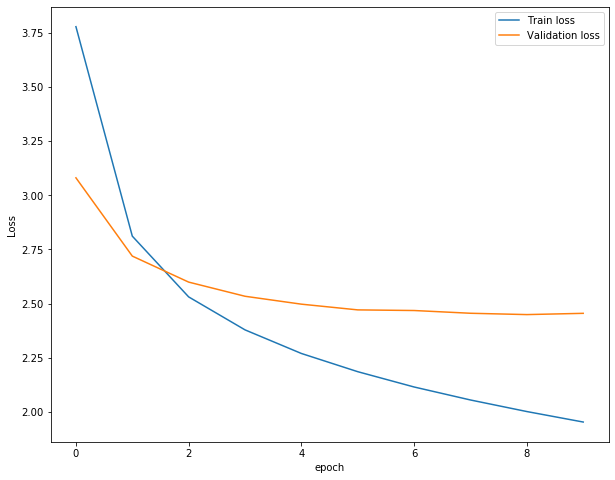
\includegraphics[width=0.8\textwidth]{LSTM_pretrainedloss}
    \caption{Training and validation loss of LSTM with pretrained embedding}
    \label{LSTM_pre_loss}
\end{figure}


\section{Experiments}
In this section, we will show the performance of our networks and discuss the reason why it performs well. There is three subsections. The first is using deterministic approach to generate captions . The second is using stochastic approach to generate captions. The Third is using pre-trained word embeddings.
\subsection{deterministic approach}

\subsection{stochastic approach}
In this section, we show the BLEU-1 and BLEU-4 socres of our models.\\
The result of the baseline model is shown in Table.\ref{baseline_table}. In the table, we can see that when Temperature = 0.1 the model performs the best. When Temperature is very little, stochastic approach is close to deterministic approach. The reason is that when Temperature is very low, the word with highest probability will equal to 1 which is quite same as the deterministic approach.

\begin{table}[htb!]
    \begin{tabular}{lllllll}
    Temperature & 0.1   & 0.2   & 0.7   & 1     & 1.5   & 2     \\
    BLEU-1      & 87.29 & 87.22 & 87.05 & 85.89 & 72.19 & 55.73 \\
    BLEU-4      & 17.3  & 17.13 & 15.41 & 13.16 & 5.66  & 3.48 
    \end{tabular}
    \caption{BLEU-1 and BLEU-4 scores of the baseline model with the stochastic approach}
    \label{baseline_table}  
\end{table}

\subsection{pre-trained word embeddings}
In this section, we show the performance of the network using pretrained word embeddings.




\begin{table}[!htb]
    \caption{BLEU-1 and BLEU-4 scores}
    \label{acc}
    \centering
    \begin{tabular}{l|c|c|}
        \hline
        model & BLEU-1 & BLEU-4 \\
		\hline
		LSTM with pretrained word embedding&87.31&19.02\\
	    \hline
    \end{tabular}

\end{table}

\section{Individual Contribution}

\subsection*{Nan Wei}
I implement transfer learning with DeepLabv3 and do experiments on basic CNN and DeepLabv3. I also write the report.

\subsection*{Renjie Shao}
I implement U-Net architecture and do experiments on U-Net. I also help implement IoU and visualization of segmentation and write some parts of the report.
\subsection*{Hongyi Ling}
I implement the generation part of our model and do experiments on baseline model.  In addition, I write these parts of the report.

\bibliographystyle{unsrt}
\bibliography{references}


\end{document}
